\documentclass[conference]{IEEEtran}
\usepackage[T1]{fontenc}
\usepackage[utf8]{inputenc}
\usepackage{amsmath,amssymb}
\usepackage{graphicx}
\usepackage{booktabs}
\usepackage{url}
\usepackage[hidelinks]{hyperref}
\hypersetup{pdftitle={Evaluating Provenance-Aware ERP Reconciliation: Fidelity, Context, and Query Parity},pdfauthor={Anonymous Review Draft},pdfsubject={Exploratory two-dataset workshop manuscript}}
\newcommand{\GraphNodes}{249,786}
\newcommand{\GraphEdges}{274,856}
\newcommand{\GraphBuildSeconds}{1.69}
\newcommand{\EdgeCoverage}{100}
\newcommand{\NodeLineage}{100}
\newcommand{\SupplierCount}{13}
\newcommand{\ItemCount}{227}
\newcommand{\SeedCount}{3}
\newcommand{\TestGroups}{49}
\newcommand{\MeanDelta}{+0.0089}
\newcommand{\MeanDeltaPoints}{+0.89}
\newcommand{\BootstrapCount}{1,000}
\newcommand{\MinCandidates}{1,314}
\newcommand{\MaxCandidates}{1,411}
\newcommand{\BlockingRecall}{100}
\newcommand{\WdcTrain}{2,500}
\newcommand{\WdcValidation}{2,500}
\newcommand{\WdcTest}{4,500}
\newcommand{\WdcBZeroFone}{0.0000}
\newcommand{\WdcBOneFone}{0.3664}
\newcommand{\WdcBTwoFone}{0.3971}
\newcommand{\QoneFone}{0.8399}
\newcommand{\SqlJoinCount}{8}
\newcommand{\LineageAuditCount}{100}
\newcommand{\QueryCount}{6}
\newcommand{\TestCount}{14}
\newcommand{\ReplicationDifference}{0.000000000000}
\newcommand{\GrowthExponent}{2.00}
\newcommand{\MaxScaleNodes}{183,590}
\newcommand{\MaxScaleCandidates}{141,100}
\newcommand{\MaxScaleMasters}{980}
\newcommand{\PeakRssGiB}{1.10}
\newcommand{\CpuCount}{24}
\newcommand{\RamGiB}{63.5}
\newcommand{\FalseMergeCount}{4}
\newcommand{\AcceptedCount}{112}
\newcommand{\AnchorCount}{51}
\newcommand{\AnchorErrors}{0}
\newcommand{\SupportedMin}{50}
\newcommand{\SupportedMax}{200}
\newcommand{\BTwoClean}{0.7606}
\newcommand{\BFiveClean}{0.7688}
\newcommand{\BTwoAttrThirty}{0.5557}
\newcommand{\BFiveAttrThirty}{0.5657}
\newcommand{\BTwoAttrFifty}{0.5254}
\newcommand{\BFiveAttrFifty}{0.5374}
\newcommand{\BTwoEdgeThirty}{0.7606}
\newcommand{\BFiveEdgeThirty}{0.7740}
\newcommand{\BTwoNoAnchors}{0.7606}
\newcommand{\BFiveNoAnchors}{0.7606}

\newcommand{\artifact}{KG-ERP}
\title{Evaluating Provenance-Aware ERP Reconciliation:\\Fidelity, Context, and Query Parity}
\author{\IEEEauthorblockN{Anonymous Review Draft}}
\begin{document}
\maketitle
\begin{abstract}
Entity reconciliation can improve cross-module answers, but a graph representation alone does not establish a matching advantage. We evaluate \artifact{}, a source-preserving prototype with typed relational context, independent inferred anchors, and non-destructive identity links. Controlled silos are generated from WideWorldImporters; WDC Products separately tests attributes. The source graph reconstructs \GraphNodes{} nodes and \GraphEdges{} relationships with complete measured coverage. Across \SeedCount{} perturbation seeds, gated context changes ambiguous held-out F1 by a mean \MeanDelta{}, with uncertainty that does not establish a reliable improvement. Six query templates exhibit exact canonical SQL/graph parity; identity-sensitive answer quality improves over a source-separated baseline. Replicated workloads reach \MaxScaleNodes{} nodes but show candidate-growth exponent \GrowthExponent{}. A fresh locked environment reproduces primary scores and query answers. The contribution is a bounded, auditable evaluation protocol, with explicit negative findings and limits of synthetic ERP evidence.
\end{abstract}
\begin{IEEEkeywords}
entity resolution, ERP data integration, provenance, knowledge graphs, reproducibility
\end{IEEEkeywords}

\section{Introduction and Positioning}
Operational modules can describe the same supplier or stock item using different identifiers and lexical forms. A permissive matcher risks combining distinct entities, while unresolved identities fragment cross-module answers. A typed knowledge graph makes business relations and decision evidence explicit, but accuracy must be separated from the information represented and from the reconciliation policy.

We ask five linked questions: can source records and foreign keys be reconstructed faithfully (RQ1); does safe context improve ambiguous matching over a learned attribute baseline (RQ2); does reconciliation improve answers when SQL and graph identities are controlled (RQ3); how does the method behave under noise (RQ4); and what workload costs and candidate growth are observed (RQ5)? We use a design-and-evaluate artifact approach consistent with design science~\cite{hevner2004}. The evaluation concerns a prototype, not a deployed ERP service.

Relational entity resolution predates this study: Bhattacharya and Getoor jointly resolve co-occurring references~\cite{bhattacharya2007}. Ditto treats matching as Transformer-based pair classification~\cite{ditto2020}, and GraphER connects graph differential dependencies to neural representation learning~\cite{grapher2025}. LIS integrates ERP, manufacturing execution, and master data using ontology mappings and validation~\cite{lis2023}. Accordingly, we claim neither the invention of contextual matching nor novelty from combining ERP and graphs. Our contribution is an inspectable evaluation chain that separates graph fidelity, context scoring, accepted identities, downstream answers, and operating costs. WDC's difficulty/unseen-entity dimensions motivate a separate external attribute check~\cite{wdc2024}.

\section{Artifact and Decision Procedure}
The artifact uses Python, NetworkX directed typed multigraphs, and indexed in-memory SQLite. SQL Server 2022 Developer supplies authentic WWI extracts and reference join counts. Record nodes retain source UID, table, local row reference, source batch, and mapper version. The raw reference graph is kept separate from model-visible silo graphs. Purchase orders point to suppliers; order lines point to orders and stock items; movements point to stock items and to orders/suppliers only where verified foreign keys permit them. Supplier transactions point to suppliers; no unsupported transaction-to-order link is created.

\begin{figure}[t]
\centering
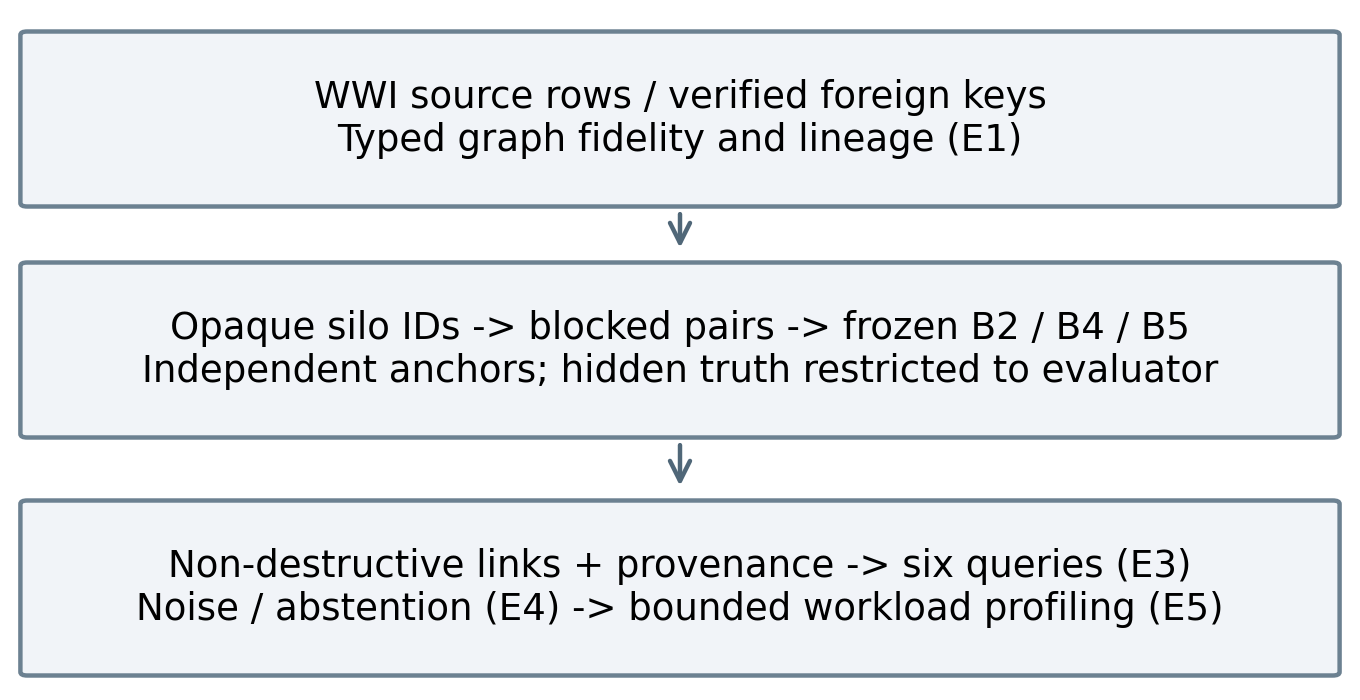
\includegraphics[width=\columnwidth]{figures/architecture.png}
\caption{WWI evaluation pipeline. WDC is an independent attribute-only E2 experiment and supplies no ERP neighborhoods.}
\label{fig:pipeline}
\end{figure}

\subsection{Attributes, Candidates, and Context}
Candidates are cross-silo, same-type pairs sharing a normalized token prefix or visible broad category. The candidate list is identical across scorers. B0 requires a nonempty normalized exact name; B1 uses validation-tuned token-sort similarity. B2 is class-balanced regularized logistic regression on fuzzy/name-token similarities, training-fitted character 3--5-gram TF-IDF, category/brand agreement, description similarity, compatible-currency price similarity, and missingness. Regularization is selected from $C\in\{0.1,1,10\}$ using validation F1, with conservative threshold tie-breaking.

Context contains supplier/stock-item neighbors and two-hop co-supplied items. Only same-partition master edges are available. Exact-normalized names that are unique in both silos, have compatible types, and lack category contradiction establish inferred anchors. No original master IDs, shared transaction keys, hidden canonical labels, or iterative match feedback are available to the scorer. Candidate endpoints cannot support themselves. Let $s_{ij}$ be the number of independently anchored neighboring correspondences, and let $a_{ij}$ and $c_{ij}$ be attribute/context vectors. Context features include anchored Jaccard, $s_{ij}$, degree similarity, category-distribution cosine, support fraction, and availability. B5 predicts
\begin{equation}
p_{ij}=\begin{cases}
\sigma(\beta_0+\beta_a^T a_{ij}+\beta_c^T c_{ij}),&s_{ij}\geq2,\\
p^{B2}_{ij},&s_{ij}<2.
\end{cases}
\end{equation}
B4 independently computes the same permitted neighborhoods with SQLite joins and applies the ungated context learner. Graph/SQL feature equality is checked. B4 versus B5 therefore compares gating as well as thresholds, not graph storage. The ungated B5 ablation is equivalent to B4's learner; the no-context ablation uses B2's probability and policy.

\subsection{Identity and Provenance}
Validation selects accept thresholds; a fixed rejection threshold defines an unresolved interval. Accepted links additionally satisfy same-type and one-to-one cross-source constraints. Original records are never rewritten or transitively unioned. The base simulation assumes one master record per entity per silo; arbitrary within-source duplicate clustering is outside scope. Each decision logs source UIDs, score, thresholds, status, model checksum, evidence references, independent anchor pairs, and decision trigger. These properties support replay. They do not constitute a PROV-O export or conformance claim~\cite{prov2013}, nor calibrated confidence or a human explainability evaluation.

\section{Experimental Protocol}
\subsection{Dataset Roles and Exploratory Status}
WWI Standard OLTP v1.0~\cite{wwi} is Microsoft's fictional enterprise sample. Six tables supply the reference graph: suppliers, purchase orders, order lines, stock items, stock movements, and supplier transactions. Its independent master population is \SupplierCount{} suppliers and \ItemCount{} stock items. Canonical groups are partitioned before aliases: supplier groups 7/3/3 and stock-item groups 136/45/46 for train/validation/test. Supplier activity is stratified using observed purchases and stock links. There are \TestGroups{} independent test groups and two separately perturbed master views. The silo graph retains all orders, lines, and supplier transactions, plus the first 5,000 primary-key-sorted movements. Accounting-like transactions occupy silo B and purchasing silo A. Native cross-silo order keys are omitted.

Initial aliases use typo probability 0.25, abbreviation probability 0.35, optional missingness 0.20, and independently removed master edges at rate 0.15. These are simulation settings, not estimated enterprise error rates. Seeds 17, 29, and 43 vary perturbation; the canonical split seed is fixed. A technical pilot stopped on WDC offer overlap. A later pilot exposed empty query oracles for inactive held-out suppliers. Both are retained. The subsequent activity-stratified protocol requires nonempty oracle tasks before model fitting and is explicitly exploratory because this construction correction followed test review. No positive-effect preregistration is claimed.

WDC uses its official pairwise 50\% corner-case, small-development, 100\%-unseen configuration, with \WdcTrain{}/\WdcValidation{}/\WdcTest{} train/validation/test pairs. Offer disjointness is verified; official pairs are not re-split. The fully unseen variant replaced the half-unseen variant before any WDC fitting because the downloaded half-unseen files contained offers shared with development data. WDC contributes attribute evidence only; cluster IDs, labels, pair IDs, and hard-negative flags are evaluator metadata.

\subsection{Outcomes and Controls}
E1 compares source/graph node and edge sets, \SqlJoinCount{} independently obtained SQL join counts, source lineage, and import idempotence. E2 freezes models before test scoring. The primary endpoint is B5 minus B2 conditional F1 on an attribute-defined ambiguous subset: name ratio below 0.95 or multiple candidates with token-sort similarity at least 0.65 for a left record. Blocking recall and all-test end-to-end recall are separate outcomes. Uncertainty uses \BootstrapCount{} paired resamples with canonical-group multiplicities on both endpoints; same-group positive pairs receive one multiplicity. These intervals are descriptive under a small, correlated simulation and are not pooled into a population confidence interval. Seed variability is reported separately.

E3 freezes six source-UID answer templates and compares unreconciled SQL (R0), predicted-identity graph (R1), SQL with exactly the same identities (R2), and an evaluator-only oracle. E4 holds clean candidates and thresholds fixed under attribute noise, edge removal, and absent anchors. E5 uses namespace-disjoint replicas, three trials per size, an explicit query warm-up, and five warmed six-template batches per trial. Timing is separated by stage; process RSS is sampled every 50 ms. Measurements use Windows 11, Python 3.12.10, \CpuCount{} logical CPUs, and \RamGiB{} GiB RAM. Replicas add workload, not independent entities.

\section{Measured Results}
\subsection{Fidelity and Primary Matching}
E1 constructs \GraphNodes{} nodes and \GraphEdges{} mapped relationships in \GraphBuildSeconds{} s for the recorded build. Node/edge precision and recall are complete in scope; expected-edge coverage is \EdgeCoverage{}\% and node lineage \NodeLineage{}\%. All SQL counts agree, no in-scope orphans occur, repeated imports preserve counts, and \LineageAuditCount{} sampled source-row checks agree.

\begin{table*}[t]
\caption{Primary ambiguous held-out F1 on identical candidates. Each seed has \TestGroups{} total held-out canonical groups; pair counts refer to the ambiguous subset. Intervals use paired entity multiplicities.}
\label{tab:primary}
\centering\begin{tabular}{rrrrrrr}
\toprule
Seed & Pairs & B2 & B4 & B5 & $\Delta$ B5--B2 & 95\% interval \\
\midrule
17 & 1304 & 0.6500 & 0.7174 & 0.6667 & +0.0167 & [-0.0784, +0.1014] \\
29 & 1383 & 0.7532 & 0.7532 & 0.7632 & +0.0099 & [+0.0000, +0.0409] \\
43 & 1403 & 0.7246 & 0.7246 & 0.7246 & +0.0000 & [+0.0000, +0.0000] \\
\bottomrule
\end{tabular}

\end{table*}

Table~\ref{tab:primary} shows mean uplift \MeanDelta{} (\MeanDeltaPoints{} F1 percentage points). The intervals include zero and effects vary by seed. The practical two-point target is not demonstrated; H2 remains inconclusive. B4 does not establish a graph representation advantage because the permitted graph and relational feature vectors are equal. The common all-test candidate counts range from \MinCandidates{} to \MaxCandidates{}, with \BlockingRecall{}\% blocking recall, so candidate-conditional and full-pipeline recall coincide for these runs.

\begin{table}[t]
\caption{WDC attribute-only test results on the official fully unseen configuration. These are independent fitted baselines, not graph-context evidence.}
\label{tab:wdc}
\centering\begin{tabular}{lrrr}
\toprule
Model & Precision & Recall & F1 \\
\midrule
B0 & 0.0000 & 0.0000 & 0.0000 \\
B1 & 0.2453 & 0.7240 & 0.3664 \\
B2 & 0.2685 & 0.7620 & 0.3971 \\
\bottomrule
\end{tabular}

\end{table}

Table~\ref{tab:wdc} reports B2 F1 \WdcBTwoFone{} versus fuzzy B1 \WdcBOneFone{}. This modest result does not establish transfer to strong neural baselines. Ditto and GraphER were not executed, so no state-of-the-art comparison is claimed. All numerical tables and narrative macros are generated from saved CSV/JSON evidence rather than manually copied.

\subsection{Queries and Error Audit}
\begin{table}[t]
\caption{Mean query-answer F1 across seeds and nonempty oracle denominators. R1 and R2 answer sets are identical for every seed/template.}
\label{tab:queries}
\centering\begin{tabular}{lrrr}
\toprule
Query & Oracle $|A|$ & R0 F1 & R1/R2 F1 \\
\midrule
Q1 & 24 & 0.0000 & 0.8399 \\
Q2 & 9 & 1.0000 & 1.0000 \\
Q3 & 2 & 0.0000 & 1.0000 \\
Q4 & 45 & 1.0000 & 1.0000 \\
Q5 & 1248 & 0.0000 & 1.0000 \\
Q6 & 3 & 0.0000 & 1.0000 \\
\bottomrule
\end{tabular}

\end{table}
Q1 links purchasing suppliers to warehouse items through order lines and resolved item identity; Q2 checks ordered versus received outers; Q3 attributes those quantities to resolved suppliers; Q4 identifies items with movements; Q5 links supplier transactions across silos; Q6 identifies supplier aliases. Q2/Q4 are source-local controls. R0 preserves distinct source IDs and performs no name-based reconciliation. Against this baseline, Q1 mean F1 reaches \QoneFone{} and the other identity-sensitive tasks are correct (Table~\ref{tab:queries}). Exact R1/R2 equality answers H3b in this scope. H3a is a reconciliation benefit relative to R0, not superiority over a SQL system using equally good identities.

The post-hoc audit distinguishes pair errors from links surviving one-to-one constraints. Across seeds, \FalseMergeCount{} of \AcceptedCount{} accepted B5 links are false merges. One size-variant shirt pair is linked despite differing hidden identities and supportive neighbors: products can share a supplier without sharing identity. All \AnchorCount{} inferred anchors agree with evaluator truth (\AnchorErrors{} observed errors), but that finding is limited to these generated views. Only \SupportedMin{}--\SupportedMax{} candidate pairs per seed satisfy the context gate.

\subsection{Robustness and Cost}
\begin{figure*}[t]
\centering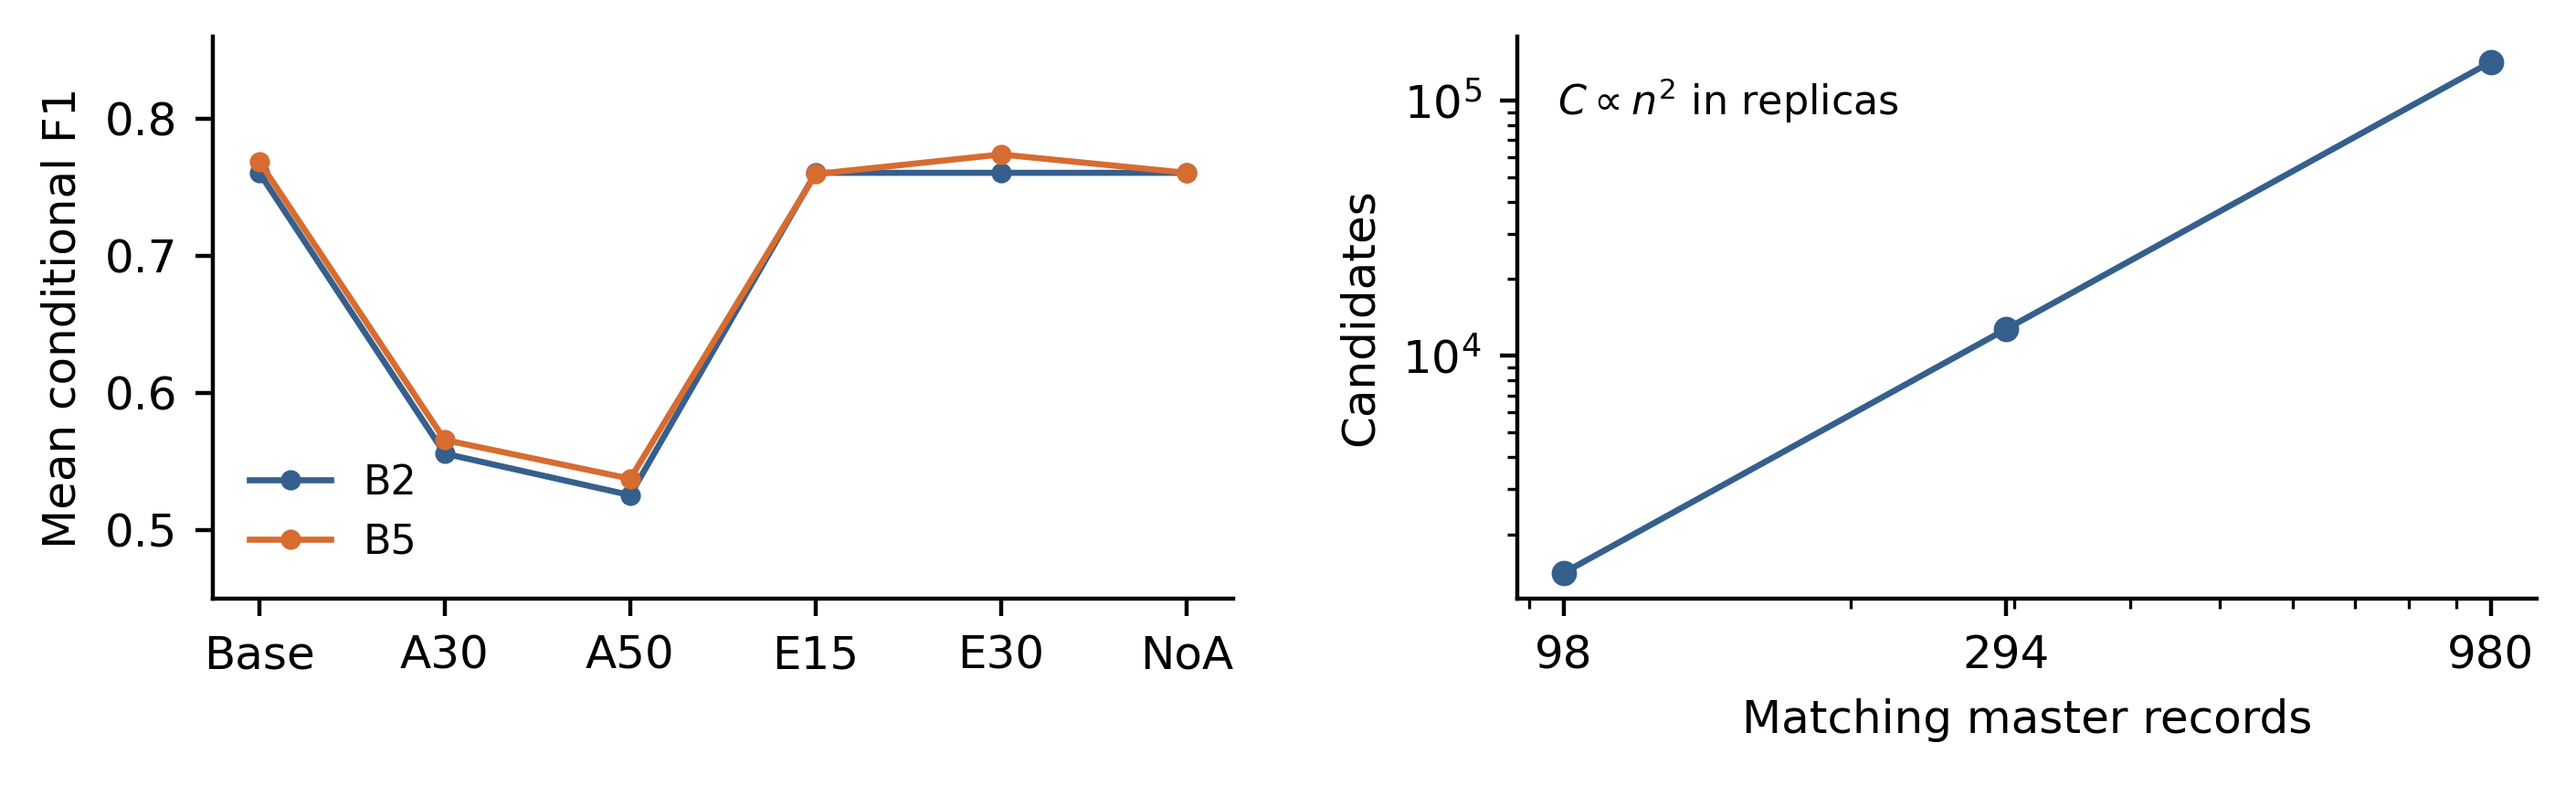
\includegraphics[width=.92\textwidth]{figures/robustness_scale.png}
\caption{Left: seed-mean conditional F1 under frozen clean candidates (A: attribute perturbation, E: additional edge removal, NoA: no anchors). Right: replicated matching workload exhibits quadratic candidate growth; replicas do not increase independent entity diversity.}
\label{fig:robustness}
\end{figure*}
Under the 50\% attribute-noise scenario, B2/B5 mean F1 is \BTwoAttrFifty{}/\BFiveAttrFifty{}, versus \BTwoClean{}/\BFiveClean{} on clean candidates. These small descriptive differences do not establish H4. The absent-anchor case yields \BTwoNoAnchors{}/\BFiveNoAnchors{}. Removing 30\% additional edges gives B5 \BFiveEdgeThirty{}, illustrating that the noise response is not necessarily monotone. Confidence-gate coverage and selective risk are logged; no calibrated probability claim is made. Adversarial edge addition and provenance-weight ablations remain untested.

\begin{table}[t]
\caption{E5 medians over three trials. SQL/KG latency is the median warmed six-query batch p50, in milliseconds. ``Masters'' counts matching test records; all source nodes are built.}
\label{tab:scale}
\centering\footnotesize\begin{tabular}{rrrrr}
\toprule
Nodes & Masters & Candidates & SQL ms & KG ms \\
\midrule
18,359 & 98 & 1,411 & 14.7 & 92.3 \\
55,077 & 294 & 12,699 & 55.3 & 208.4 \\
183,590 & 980 & 141,100 & 255.8 & 616.8 \\
\bottomrule
\end{tabular}

\end{table}

Table~\ref{tab:scale} reaches \MaxScaleNodes{} nodes, \MaxScaleMasters{} matching records, and \MaxScaleCandidates{} candidates. The fitted candidate exponent is \GrowthExponent{}, failing H5's below-quadratic target for replicated descriptions. Maximum sampled process RSS is \PeakRssGiB{} GiB. Unique-name anchors disappear as descriptions are replicated. SQL indexes are built once; the current graph query routine rebuilds adjacency per batch. The latency gap therefore describes implementation costs, not an intrinsic graph-versus-SQL property or enterprise-scale feasibility.

\section{Reproducibility, Limits, and Conclusion}
A newly created environment installs the complete dependency lock, passes \TestCount{} control tests, regenerates aliases, retrains each WWI seed on train/validation only, and reproduces frozen probabilities, thresholds, accepted decisions, and all query answers within the declared $10^{-12}$ tolerance. WDC attribute retraining also agrees. Input, code, model, and result checksums are retained; replay does not retune on test. E5 timings are not expected to reproduce exactly across cache or hardware conditions.

The study provides faithful in-scope construction evidence for RQ1; inconclusive contextual uplift for RQ2; measured reconciliation benefit and exact representation parity for RQ3; descriptive, limited robustness evidence for RQ4; and a negative candidate-growth finding for RQ5. It lacks independent dirty ERP sources, a production deployment, strong neural comparisons, adversarial relation tests, and a human explanation study. Groups are few, silos share an original database, one-to-one identity assumptions are restrictive, and public-source distribution terms need review before releasing any data/model bundle. Further performance-driven changes must remain exploratory and versioned.

\artifact{} supplies an auditable prototype and evaluation chain, not evidence that graph storage alone improves entity resolution. The supported lesson is to retain source provenance, measure context against equivalent relational information, and verify downstream answers under shared identities. Negative matching and scaling findings are part of the result. An independent-source study is needed before broader ERP claims.

\IEEEtriggeratref{2}
\bibliographystyle{IEEEtran}
\bibliography{references}
\end{document}
